\section{System Setup}
A system is provided by the automation and control department at Aalborg University (AAU). The setup is seen in \autoref{fig:systemSetup}, the parameters that can be measured directly are indicated.

\begin{figure}[H]
  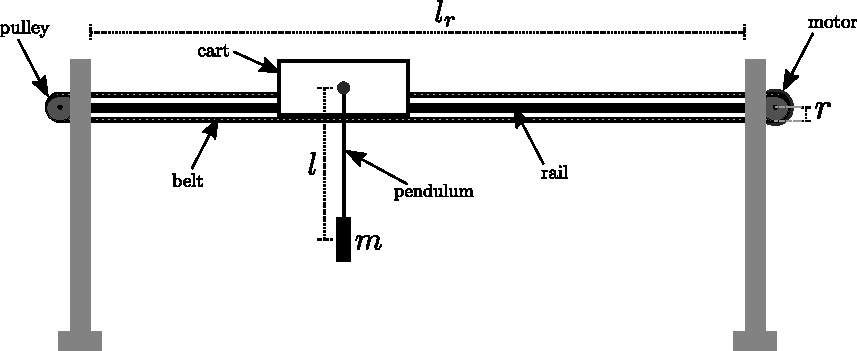
\includegraphics[width=.8\textwidth]{figures/systemSetup}
  \caption{The system setup provided by AAU, where $m$ is the mass of the pendulum weight attached at the end of the rod, $l$ is the length from pivot point to center of mass, $r$ is the radius of the pulley and $l_r$ is the effective length of the rail.}
  \label{fig:systemSetup}
\end{figure}

The mass of the cart cannot be directly measured as it is preferred not to take the system apart. This parameter is later estimated along with frictions in the system.

